\subsubsection*{Background}

Active matter has been a field of rapidly expanding interest and research activity over the last decade \cite{Ramaswamy_2010_AnnRevConMatPhys,MarchettiEA_2013_RevModPhys,BechingerEA_2016_RevModPhys,MarchettiEA_2016_CurrentOpinionColloidInterfaceScience}.
Vicsek's pioneering work showed that collections of point particles with alignment rules displayed rich collective behavior, including phase separation \cite{VicsekEA_1995_PRL}.
However, theoretical work seeking to describe the collective behavior of bacteria demonstrated that phase separation was not reliant upon explicit alignment rules \cite{Cates_2010_PNAS}.
Giant number fluctuations characteristic of phase separation in these systems of isotropic particles were found to lead to phase separation based on density-dependent slowing in a phenomena now known as ``motility-induced phase separation'' (MIPS) \cite{CatesTailleur_2013_EPL}. 
This phase separation in isotropic systems has been described as athermal phase separation \cite{FilyMarchetti_2012_PRL}, kinetic steady-state balancing of particle fluxes \cite{RednerEA_2013_PRE, RednerEA_2013_PRL}, classical nucleation \cite{Richard_2016_SoftMatter,Redner_2016_PRL}, and balancing of collision theory timescales \cite{Bruss_2017_arxiv}.
Importantly, this same phase separation predicted by theory has been observed in experiments, which confirm the activity-dependent formation of ``active crystals'' at low system densities \cite{PalacciEA_2013_Science,PetroffEA_2015_PRL}.

However, in real-world systems (e.g. bacteria) particles are rarely isotropic.
Simulations of rods with varying aspect ratios have been shown to display a rich variety of collective motion dependent on shape and system density \cite{WensinkLoewen_2012_JPhysConMat,YangEA_2010_PRE}.
Drawing from the example of anisotropic swimmers such as bull sperm and \textit{Chlamydomonas}, Wensink \textit{et al} observed that shape and direction of the translational driving force relative to the shape (referred to as ``force offset'' in this paper) allowed for differing modes of collective motion and onset of critical behavior \cite{Wensink_2014}.
Similarly, gear shaped ``spinners'' with differing directions of a rotational driving force were shown to phase separate through competing steric interactions (repulsive for opposite spinners, and attractive for like spinners) \cite{NguyenEA_2014_PRL, SabrinaEA_2015_SoftMatter, SpellingsEA_2015_PNAS}.
In a study of active dumbbells, Suma \textit{et al} noted that particle anisotropy allowed for stabilization of cluster rotation, a phenomenon not seen in clusters of isotropic particles \cite{SumaEA_2014_EPL}.
Finally, a study of active squares uncovered an ``oscillatory'' activity/density regime in which large clusters would break up and re-form at steady state \cite{PrymidisEA_2016_SoftMatter}. 

Why is a description of the role of active particle anisotropy needed?
We can view this spontaneous ``phase separation'' and organization as a type of non-equilibrium self-assembly \cite{Mann_2009_NatureMaterials}.
It is well established that in the absence of attractive forces in equilibrium self-assembly, shape alone is sufficient to determine the minimum free-energy structure \cite{Onsager_1949_ANYAS,Damasceno_2012_Science,Manoharan_2015_Science,vanAndersEA_2014_PNAS}. 
While self-assembling, fluctuations allow a system to randomly sample system configurations until it finds the one with the minimum free energy.
However, sometimes the global free energy minimum is kinetically difficult to reach, and the system can become kinetically trapped in a metastable state.
Activity provides a driving force which can help anneal a system out of these kinetic traps \cite{VanDerMeerDijkstraFilion_2016_SoftMatter,Mallory_2016_PRE} or stabilize system configurations that would be unstable without the additional driving force \cite{ZhangYanEA_2016_AngewandteChemie}. 
Understanding how particle anisotropy combined with an active force director will impact the collective motion, even in the form of a general heuristic, would open the doors to studying non-equilibrium self-assembly tailored through particle anisotropy. 

\begin{figure}[t]
\begin{center}
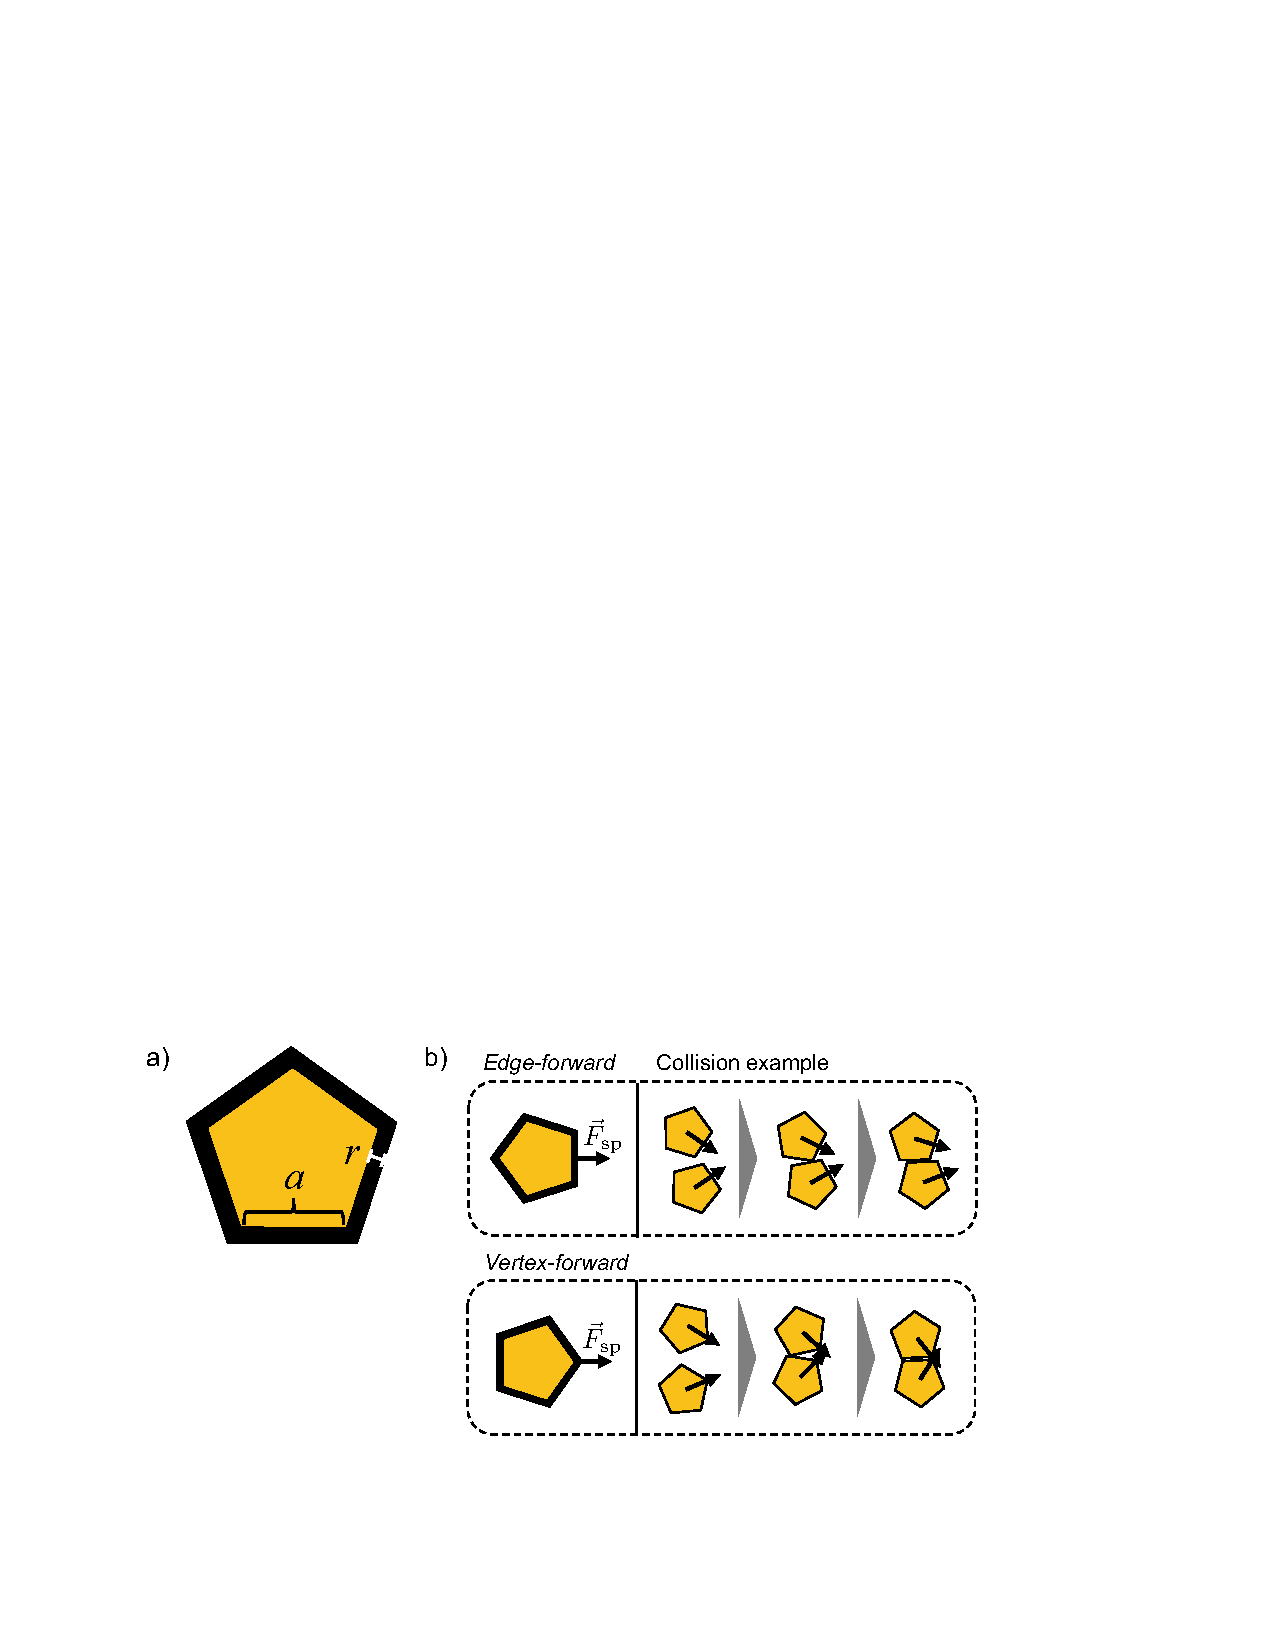
\includegraphics[width=4in]{../Figures/Fig1.pdf}
\label{fig:model}
\end{center}
\caption{
\textbf{Model system}:
(a) Shape anisotropy is studied with a family of regular polygons of side number $n=3-8$, characterized by side length $a$.
Particles interact through a purely repulsive WCA potential of radius $r=1$.
The dimensions of all shapes are set such that $\frac{n{\cdot}a}{2{\pi}r}=0.9$.
(b) Force anisotropy is implemented through the direction of the self-propelling force, which propels the shape either edge- or vertex-forward.
A key feature of this system is that collisions of anisotropic particles can sustain dimer (and larger n-mer) translational and/or rotational motion.
Illustrative collisions are provided for each force director.
}
\end{figure}

%In all studies of active shapes, some degree of particle ordering has been found in the clusters. 
To date, the differing behavior between active disks and active shapes has been explained in system-specific terms. 
Here, we study a system of active shapes to systematically understand and describe the role both shape and force anisotropy play in the collective behavior of translationally-driven active systems using the model shown in Fig. \ref{fig:model}.
Shapes are implemented using the discrete element method \cite{DEM_2017} implemented in HOOMD-blue \cite{HOOMD_2008, HOOMD_2015}.
We use Langevin dynamics to model the movement of the particles studied here, and take care to select a sufficiently small mass that the system is effectively Brownian, in line with the expected dynamics of bacteria.
Full simulation parameters can be found in the Methods section of the in-preparation paper.